\normalfalse \difficiletrue \tdifficilefalse
\correctionfalse

%\UPSTIidClasse{11} % 11 sup, 12 spé
%\newcommand{\UPSTIidClasse}{11}

\exer{Mouvement RR 3D  $\star\star$ \label{C1:05:07:PFD}}
\setcounter{numques}{0}
\UPSTIcompetence[2]{B2-14}
\UPSTIcompetence[2]{C1-05}
\index{Compétence B2-14}
\index{Compétence C1-05}
\index{Principe fondamental de la dynamique}
\index{PFD}
\index{Mécanisme à 2 rotations 3D}
\ifcorrection
\else
\textbf{Pas de corrigé pour cet exercice.}
\fi

\ifprof
\else
Soit le mécanisme suivant. On a $\vect{AB}=R\vect{i_1}$ et $\vect{BC}=\ell\vect{i_2}+r\vect{j_2}$. On note $R+\ell=L = \SI{20}{mm}$ et $r=\SI{10}{mm}$. De plus :
\begin{itemize}
\item $G_1=B$ désigne le centre d'inertie de \textbf{1}, on note $m_1$ la masse de \textbf{1};% et $\inertie{G_1}{1}=\matinertie{A_1}{B_1}{C_1}{0}{0}{0}{\bas{1}}$; 
\item $G_2$ désigne le centre d'inertie de \textbf{2} tel que  $\vect{BG_2}=\ell\vect{i_2}$, on note $m_2$ la masse de \textbf{2}.% et $\inertie{G_2}{2}=\matinertie{A_2}{B_2}{C_2}{0}{0}{0}{\bas{2}}$.
\end{itemize}

Un moteur électrique positionné entre \textbf{0} et \textbf{1} permet d'actionner le solide \textbf{1}.
Un moteur électrique positionné entre \textbf{1} et \textbf{2} permet d'actionner le solide \textbf{2}.
L'accélération de la pesanteur est donnée par $\vect{g}=-g\vect{j_0}$.

\begin{center}
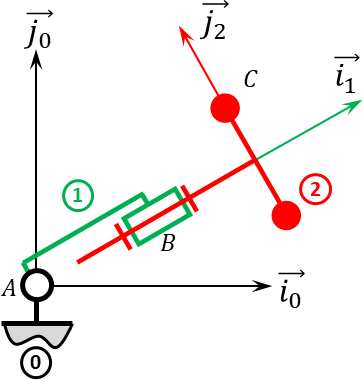
\includegraphics[width=\linewidth]{07_RR3D_01}
\end{center}
\fi

\question{Réaliser le graphe d'analyse en faisant apparaître l'ensemble des actions mécaniques.}
\ifprof
\else
\fi

\question{Proposer une démarche permettant de déterminer les loi de mouvement de \textbf{1} et de \textbf{2} par rapport à $\rep{0}$.}
\ifprof
\else
\fi

\ifprof
\else
\begin{flushright}
\footnotesize{Corrigé  voir \ref{C1:05:07:PFD}.}
\end{flushright}%
\fi